\documentclass[aspectratio=169,10pt]{beamer}
\usetheme{default}
\usecolortheme{dove}
\setbeamertemplate{navigation symbols}{}
\usepackage{booktabs}
\usepackage[T1]{fontenc}
\usepackage{graphicx}
\usepackage{lmodern}
\setbeamerfont{block body}{size=\small}
\def\evidencetext{}
\setbeamertemplate{footline}{%
  \leavevmode\hbox to \paperwidth{\hspace{0.4cm}\parbox[b]{0.86\paperwidth}{\raggedright\tiny\color{gray}%
  \ifx\evidencetext\empty\else Evidence: \evidencetext\fi}\hfill{\tiny\color{gray}\insertframenumber}\hspace{0.4cm}}\vspace{0.18cm}}
\title{PET recovery: diagnosis and improvement campaign}
\subtitle{Campaign comparison deck, version 2 (generated from committed results)}
\author{PET improvement campaign}
\date{\parbox{0.8\linewidth}{\centering\small PET is diagnostic method development. Nothing here is a publication adoption, and nothing here changes the historical comparison's verdict or thresholds.}}

\begin{document}

\gdef\evidencetext{}
\frame{\titlepage}

\gdef\evidencetext{\texttt{../configuration\_comparison/campaign\_report.json}}
\begin{frame}{The question, and the historical result}
The completed matched comparison injected a known truth $E_{\mathrm{avail}}$ tilt (amplitude 0.35)
into simulated pseudodata and scored the seven-bin recovery of the injected displacement.
\begin{center}
{\small
\begin{tabular}{lrrc}
\toprule
arm & mean recovery & adequacy floor & adequate \\
\midrule
our production PET & 0.3037 & 0.5560 & no \\
Gregor's pretrained PET2-small & 0.4165 & 0.5560 & no \\
\bottomrule
\end{tabular}}
\end{center}
Floor $= 0.8\times$ an acceptance reference 0.6950 built from $1-(1-a)^k$ at $k=3$.
Paired \texttt{ours $-$ theirs} $= \ensuremath{-}0.1129$, 95\,\% interval $[\ensuremath{-}0.1471,\,\ensuremath{-}0.0786]$, $n=8$ seed pairs;
his arm scored better in 8 of 8 pairs.
\begin{block}{Verdict (preserved, unchanged by this campaign)}
\texttt{NEITHER\_ELIGIBLE / NO\_SELECTION}. Non-inferiority margin 0.02 and switching margin 0.04 are the historical
ones and are used unchanged for every like-for-like statement below.
\end{block}
\textbf{This campaign asks:} what caused the shortfall, what fixes it, whether more events help,
whether the adequacy reference is appropriate, and what limits remain.
\end{frame}

\gdef\evidencetext{\texttt{phase\_a/receipts/runtime\_audit\_theirs.json}; \texttt{phase\_a/receipts/historical\_receipts.json}}
\begin{frame}{What actually ran (Phase A audit)}
Captured at runtime while the historical code ran unmodified through the guard (Phase A).
\begin{columns}[T]
\begin{column}{0.5\linewidth}
\textbf{1. Gregor's declared optimizer never ran.}\par\vspace{2pt}
{\small Declared: TorchAdamW with weight decay, warmup/cosine schedule, global-norm clipping.\\
Executed at step 1: \texttt{Adam} from \texttt{horovod.\_keras} (Horovod-wrapped: yes);
\texttt{weight\_decay} None, \texttt{global\_clipnorm} None, schedule object: no,
$\epsilon$ = \ensuremath{1\times10^{-7}}.\\
The intended unit global-norm clip would have bound on 100\,\% of updates (pre-clip norms up to 1474).}
\end{column}
\begin{column}{0.48\linewidth}
\textbf{2. The ``identical'' step 2 was not identical.}\par\vspace{2pt}
{\small
{\footnotesize
\begin{tabular}{lrr}
\toprule
step 2, final stage & theirs & ours \\
\midrule
batch size & 2048 & 512 \\
engine steps at gen & 586 & 2344 \\
iteration-0 learning rate & \ensuremath{1\times10^{-4}} & \ensuremath{4\times10^{-4}} \\
\bottomrule
\end{tabular}}\par\vspace{3pt}
4$\times$ more optimizer updates per epoch for ours, and a different validation subset
(the engine cuts train/validation in batches).}
\end{column}
\end{columns}
\vspace{4pt}
\begin{alertblock}{Defects of fidelity, not established causes}
These bias the between-arm comparison; they are not shown to cause the recovery shortfall.
The campaign therefore rebuilt the path with explicit per-step recipes; the repaired driver refuses
to train when the executed optimizer differs from the declared one.
\end{alertblock}
\end{frame}

\gdef\evidencetext{\texttt{phase\_b/scalar/results/summary.json}; \texttt{../configuration\_comparison/campaign\_report.json}}
\begin{frame}{Where recovery is lost (1): scalar references}
\begin{columns}[T]
\begin{column}{0.52\linewidth}
{\small At $k=3$, on the same endpoint (DEV halves; the historical closure reproduced
bit-exactly, 31 checks agree: yes):}\par\vspace{3pt}
{\scriptsize
\begin{tabular}{lr}
\toprule
estimator & recovery \\
\midrule
binned IBU, muon kinematics only & 0.164 \\
binned IBU, muon + reco $E_{\mathrm{avail}}$ & 0.472 \\
GBDT OmniFold, muon only & 0.140 \\
GBDT OmniFold, + reco $E_{\mathrm{avail}}$ & 0.412 \\
MLP OmniFold, + all reco hadronic summaries & 0.486 \\
\textbf{historical PET, ours} & \textbf{0.304} \\
\textbf{historical PET, Gregor's arm} & \textbf{0.417} \\
\bottomrule
\end{tabular}}\par\vspace{4pt}
{\small \textbf{No response-aware scalar estimator reaches the 0.556 floor at $k=3$.}
The shortfall is not PET-specific. Recovery is still climbing: IBU reaches 0.648 at
$k=10$ and 0.683 at $k=15$; GBDT 0.524 at $k=20$.}
\end{column}
\begin{column}{0.46\linewidth}
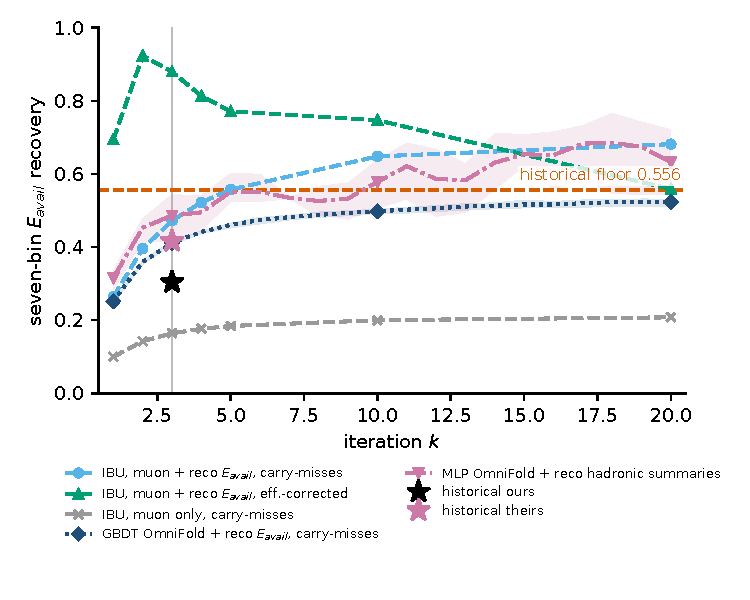
\includegraphics[width=0.95\linewidth]{figures_campaign/scalar_recovery_vs_k.pdf}
\end{column}
\end{columns}
\end{frame}

\gdef\evidencetext{\texttt{phase\_b/pet/results/summary.json}; \texttt{phase\_b/pet/results/b2e3-H-K10-s\{1,2\}.scores.json}; \texttt{phase\_b/scalar/results/summary.json}}
\begin{frame}{Where recovery is lost (2): step by step inside the unfolding}
\begin{columns}[T]
\begin{column}{0.5\linewidth}
{\small \textbf{The truth-side PET is not the bottleneck.} Given the known tilt alone it learns it to
0.898 (raw PDG codes), 0.952 (one-hot PDG), 0.973 (+ true $E_{\mathrm{avail}}$, $q_3$),
against 0.33 for any learner restricted to true muon $p_T, p_\parallel$
(and 0.999 given true $E_{\mathrm{avail}}$).\par\vspace{3pt}
\textbf{Step 1 is not either:} the pull closes reco $E_{\mathrm{avail}}$ to 0.656 after one
iteration, 0.940 by $k=10$.\par\vspace{3pt}
\textbf{The loss is in the misses and in stopping at $k=3$.} Under carry-misses every missed event
(58\,\% of the truth sample) enters step 2 with its previous weight; over accepted events
the pull holds 0.591 at $k=1$, the push keeps 0.313.}
\end{column}
\begin{column}{0.49\linewidth}
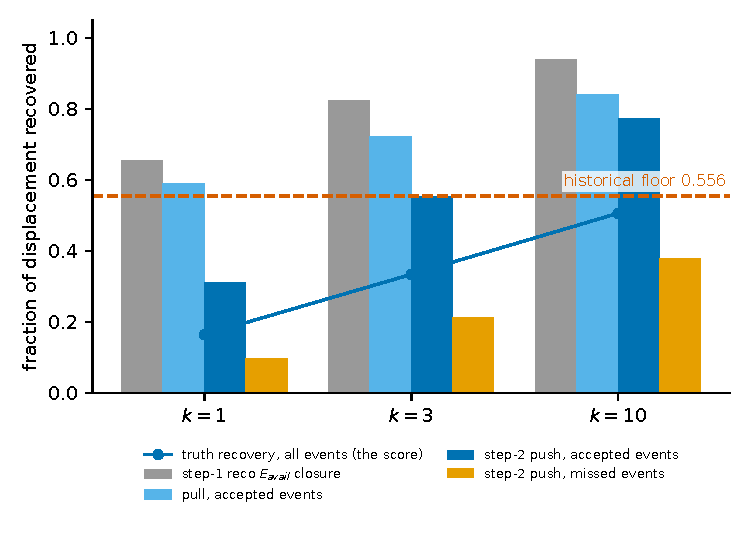
\includegraphics[width=0.95\linewidth]{figures_campaign/stepwise_closure.pdf}\\
{\scriptsize
\begin{tabular}{rrrrrr}
\toprule
$k$ & push & pull & reco $E_{\mathrm{av}}$ & acc. & missed \\
\midrule
1 & 0.164 & 0.191 & 0.656 & 0.313 & 0.098 \\
3 & 0.334 & 0.363 & 0.824 & 0.554 & 0.212 \\
10 & 0.506 & 0.512 & 0.940 & 0.774 & 0.378 \\
\bottomrule
\end{tabular}}
\end{column}
\end{columns}
\end{frame}

\gdef\evidencetext{\texttt{phase\_b/pet/results/summary.json}; \texttt{phase\_b/pet/results/b2e\{3,4\}-*-K10-s\{1,2\}.scores.json}}
\begin{frame}{What improves it (1): iterations and the miss rule; the schedule does not}
\begin{columns}[T]
\begin{column}{0.6\linewidth}
{\small PET through the repaired driver, DEV halves, $K=10$, 2 seeds, paired against H
(carry-misses, rate forced to \ensuremath{1\times10^{-5}} after iteration 0, last epoch handed on); per-seed $\Delta$ in brackets:}\par\vspace{3pt}
{\scriptsize
\begin{tabular}{lrrrl}
\toprule
factor & $k=3$ & $k=10$ & $\Delta$, $k=10$ & per seed \\
\midrule
H: historical recipe & 0.334 & 0.506 & --- &  \\
S1: no forced rate & 0.326 & 0.496 & \ensuremath{-}0.010 & [+0.021, \ensuremath{-}0.041] \\
S2: best-val.\ epoch & 0.290 & 0.452 & \ensuremath{-}0.054 & [\ensuremath{-}0.047, \ensuremath{-}0.062] \\
\textbf{M: eff.-corr.\ step 2} & 0.608 & 0.817 & +0.310 & [+0.330, +0.290] \\
\bottomrule
\end{tabular}}\par\vspace{4pt}
{\small \textbf{Iterations and the miss rule are the two levers.} Efficiency correction clears the
historical floor already at $k=3$ and lifts the low-acceptance region from 0.17 to
0.67 at $k=10$. \textbf{The schedule does not help}: handing on the best-validation
epoch \emph{hurts}.}
\end{column}
\begin{column}{0.38\linewidth}
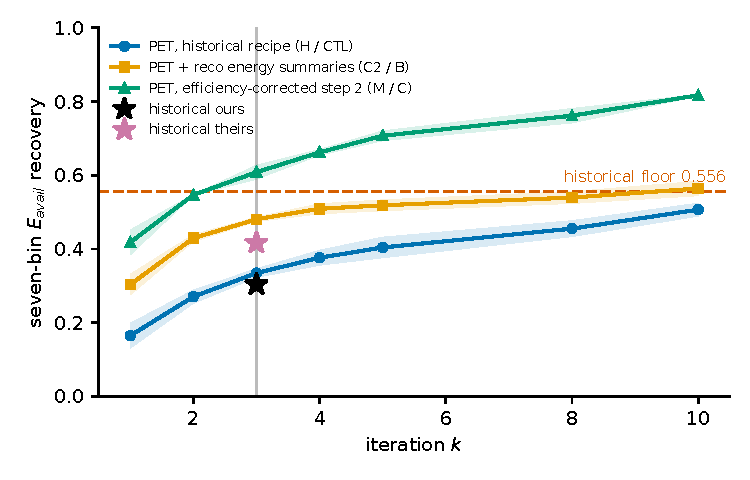
\includegraphics[width=0.95\linewidth]{figures_campaign/pet_recovery_vs_k.pdf}\\
{\scriptsize Bands: min--max over seeds. Efficiency correction is a model-dependence choice; see
the robustness slides.}
\end{column}
\end{columns}
\end{frame}

\gdef\evidencetext{\texttt{phase\_b/pet/results/summary.json}; \texttt{phase\_b/pet/results/b2e5-C\{1..4\}-H-s\{1,2\}.scores.json}}
\begin{frame}{What improves it (2): reconstructed-energy summaries at step 1}
{\small Feature arms: carry-misses, one-hot PDG truth side, $K=10$, 2 seeds, paired against C1
(per-seed $\Delta$ in brackets).}
\begin{center}
{\footnotesize
\begin{tabular}{lrrll}
\toprule
arm & $k=3$ & $k=10$ & paired $\Delta$, $k=3$ & paired $\Delta$, $k=10$ \\
\midrule
C1 incumbent inputs & 0.369 & 0.525 & --- & --- \\
\textbf{C2 + reco energy summaries at step 1} & 0.480 & 0.564 & +0.112 [+0.106, +0.117] & +0.039 [+0.040, +0.038] \\
C3 + true $E_{\mathrm{avail}}$, $q_3$ at step 2 & 0.384 & 0.544 & +0.015 [+0.011, +0.020] & +0.019 [+0.010, +0.028] \\
C4 both & 0.480 & 0.558 & +0.112 [+0.097, +0.126] & +0.032 [+0.033, +0.032] \\
\bottomrule
\end{tabular}}
\end{center}
\begin{itemize}\small
\item \textbf{Explicit reconstructed-energy summaries at the detector step are the one input change that pays}:
they speed convergence and lift the accepted events' truth recovery to 0.92 at $k=10$.
\item They do not help the missed events (0.38--0.41 in every arm at $k=10$), so
under the engine's miss rule no feature arm reaches the floor at $k=3$.
\item Truth summaries add little: the truth side already extracts $E_{\mathrm{avail}}$ from the cloud.
\end{itemize}
\end{frame}

\gdef\evidencetext{\texttt{phase\_f/results/aussie\_ablation.json}; \texttt{phase\_b/scalar/results/summary.json}}
\begin{frame}{What improves it (3): miss handling, not the non-iterative form}
{\small A bounded scalar benchmark of AUSSIE (arXiv:2602.24282), the non-iterative replacement for
OmniFold's pull step. Its first, confounded result was dissected by ablation (DEV populations):}
\begin{center}
{\footnotesize
\begin{tabular}{llcrr}
\toprule
estimator & miss handling & setting & aggregate recovery & seeds \\
\midrule
scalar OmniFold (HGB) & carry-misses (the engine's rule) & $k=50$ & 0.582 & 2 \\
scalar OmniFold (HGB) & efficiency-corrected & $k=50$ & 0.783 & 2 \\
AUSSIE & misses pinned to the prior ($\lambda=1000$) & --- & 0.648 & 3 \\
AUSSIE & unconstrained ($\lambda=0$) & --- & 0.849 & 3 \\
\bottomrule
\end{tabular}}
\end{center}
\begin{itemize}\small
\item \textbf{Most of the apparent gain is miss handling}: letting the learned ratio extrapolate to
events that fail reconstruction is worth +0.20 (AUSSIE) and +0.20
(OmniFold); AUSSIE keeps a modest edge (+0.07) at matched miss handling.
\item A PET-backbone AUSSIE evaluation is \textbf{not justified} on this evidence.
\item Efficiency correction is not free: binned IBU with the acceptance division peaks at
0.923 ($k=2$) and is back to 0.559 at $k=20$
with low-acceptance recovery \ensuremath{-}0.424. It needs a stopping rule and a variance statement.
\end{itemize}
\end{frame}

\gdef\evidencetext{\texttt{phase\_d/results/scalar\_scaling.json}}
\begin{frame}{Does more data help? (Phase D, development stage)}
{\small \textbf{Development-stage evidence} (scalar, DEV halves, 222 runs, overlapping draws
per size, a per-subset oracle anchor). The confirmatory study on fresh pool-S draws is separate.}\par\vspace{2pt}
\begin{columns}[T]
\begin{column}{0.52\linewidth}
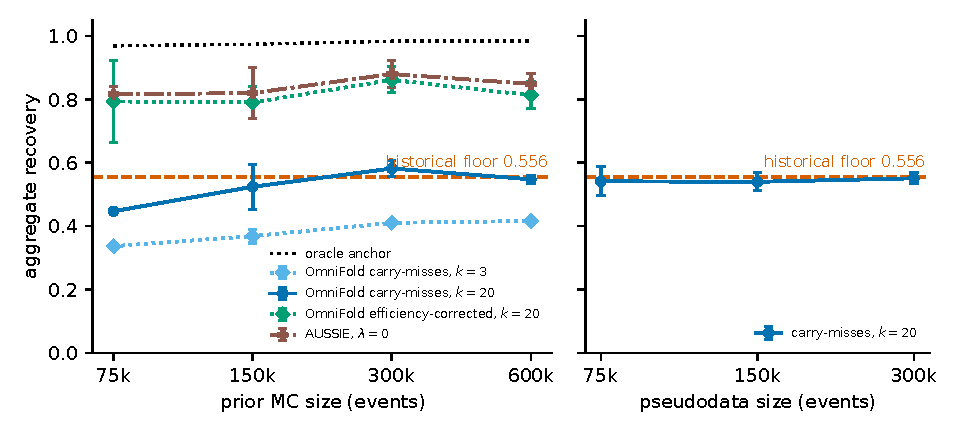
\includegraphics[width=0.95\linewidth]{figures_campaign/scaling.pdf}
\end{column}
\begin{column}{0.46\linewidth}
\begin{itemize}\footnotesize
\item Prior-MC statistics buy recovery in the historical miss mode (+0.080 at $k=3$,
+0.101 at $k=20$, 75k$\to$600k); beyond 600k is not measured.
\item Pseudodata statistics are not the binding constraint over this range.
\item Miss handling outweighs every statistical axis tested (+0.27 at 600k).
\item Error bars: sd over draws.
\end{itemize}
\end{column}
\end{columns}
\vspace{-2pt}
\begin{center}
{\tiny
\begin{tabular}{lrrrr}
\toprule
axis (aggregate recovery) & 75k & 150k & 300k & 600k \\
\midrule
OmniFold carry-misses, $k=3$ & 0.337 & 0.369 & 0.411 & 0.416 \\
OmniFold carry-misses, $k=20$ & 0.447 & 0.524 & 0.582 & 0.548 \\
OmniFold efficiency-corrected, $k=20$ & 0.794 & 0.791 & 0.862 & 0.813 \\
AUSSIE, $\lambda=0$ & 0.816 & 0.820 & 0.880 & 0.849 \\
pseudodata size: carry-misses, $k=20$ & 0.541 & 0.540 & 0.551 & --- \\
oracle anchor (exact tilt on that subset) & 0.969 & 0.974 & 0.984 & 0.984 \\
\bottomrule
\end{tabular}}
\end{center}
\end{frame}

\gdef\evidencetext{\texttt{phase\_b/scalar/results/reference\_decomposition.json}; \texttt{phase\_b/scalar/results/summary.json}; \texttt{../configuration\_comparison/campaign\_report.json}}
\begin{frame}{The adequacy reference (1): what it measures}
\begin{columns}[T]
\begin{column}{0.5\linewidth}
{\footnotesize The reference is $1-(1-a)^k$ at $k=3$ with a per-cell acceptance $a$; the floor is
0.8$\times$ it.\par\vspace{3pt}
\textbf{It is computed on a different quantity from the one scored.} It is built on the
$(p_T, p_\parallel)$ cell displacement (0.695); the score is the seven-bin $E_{\mathrm{avail}}$ marginal.
The model's own assumptions applied to the scored spectrum give 0.578; on the actual halves with the
historical pseudodata normalization, 0.523: \emph{below the 0.556 floor derived from it.}\par\vspace{3pt}
\textbf{It is not an attainability bound in either direction.} Efficiency-corrected IBU exceeds it
(0.923 at $k=2$) and recovers the low-acceptance region (reference 0.014) at
0.76, but only by dividing by acceptance, which the engine's miss rule never does.\par\vspace{3pt}
The historical normalization assumes the accepted fraction is unchanged by the tilt; measured ratio
0.8979.}
\end{column}
\begin{column}{0.48\linewidth}
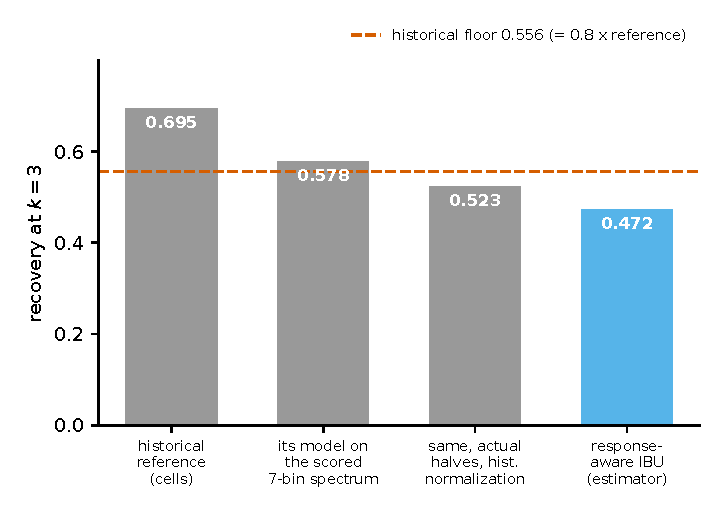
\includegraphics[width=0.95\linewidth]{figures_campaign/reference_decomposition.pdf}
\end{column}
\end{columns}
\end{frame}

\gdef\evidencetext{\texttt{phase\_e/results/reference\_assessment.json}; \texttt{phase\_e/results/toy\_reference.json}}
\begin{frame}{The adequacy reference (2): a definitional gap}
{\small \textbf{The gap is definitional, not statistical} (fresh pool-S events, 3 replicates per size):}
\begin{center}
{\footnotesize
\begin{tabular}{lrr}
\toprule
quantity at $k=3$ & historical size & 8$\times$ the events \\
\midrule
historical reference model (rebuilt on pool S) & 0.6950 & --- \\
response-aware IBU, $k=3$ & 0.472 & 0.480 \\
reference model realized on the scored object & 0.523 & 0.528 \\
\bottomrule
\end{tabular}}
\end{center}
{\small Eight times the statistics closes 0.008 of the 0.223 gap: at least
96\,\% of it comes from what the reference assumes, not from sample size.\par\vspace{4pt}
\textbf{A known-function toy} (no smearing): $1-(1-a)^k$ at $k=3$ gives 0.788; the engine's miss rule
attains 0.659 (0.025 of the gap from the score's renormalization, 0.104 from the
engine's normalization); efficiency correction reaches 0.991, above it. Neither a bound nor a match.}
\begin{block}{Prospective recommendation only (not adopted; changes no verdict)}
\small A reference must be computed for the estimator's actual miss rule and normalization, on the scored
seven-bin spectrum, and a floor derived from it checked on a known-function toy before use. The historical
thresholds are retained unchanged for every like-for-like verdict in this campaign.
\end{block}
\end{frame}

\gdef\evidencetext{\texttt{phase\_e/results/identifiability.json}}
\begin{frame}{Robustness (1): what the data can distinguish}
{\small A reco-level two-sample classifier at the historical pseudodata size; null from
20 equal-model splits: mean +0.0002, 95\,\% band
[\ensuremath{-}0.0019, +0.0020]. Fresh pool-T events.}\par\vspace{4pt}
\begin{columns}[T]
\begin{column}{0.47\linewidth}
\small \textbf{Every predeclared truth distortion is distinguishable} (23 of
23), by 2.6\ensuremath{\times} to 62.5\ensuremath{\times} its own ESS-scaled threshold.
The weakest is D4d (neutron multiplicity), the hidden-variable test.\par\vspace{4pt}
The $\pm5\,\%$ hadronic scale (R1) is distinguishable. The $\pm1\,\%$ muon scale (R2) sits at or below
threshold and the cluster smearing (R3) is not distinguishable: \textbf{unprobed at this size, not harmless}.
\end{column}
\begin{column}{0.5\linewidth}
{\footnotesize
\begin{tabular}{lrrc}
\toprule
case & AUC$-\frac{1}{2}$ & threshold & disting. \\
\midrule
\texttt{D4d\_n\_up} & +0.0126 & 0.0023 & yes \\
\texttt{D4d\_n\_down} & +0.0055 & 0.0022 & yes \\
\texttt{R1\_x1.05} & +0.0218 & 0.0021 & yes \\
\texttt{R1\_x0.95} & +0.0241 & 0.0021 & yes \\
\texttt{R2\_x1.01} & +0.0023 & 0.0021 & yes \\
\texttt{R2\_x0.99} & \ensuremath{-}0.0002 & 0.0021 & no \\
\texttt{R3\_s0.10} & \ensuremath{-}0.0014 & 0.0021 & no \\
\bottomrule
\end{tabular}}
\end{column}
\end{columns}
\end{frame}

\gdef\evidencetext{\texttt{phase\_e/results/references.json}; \texttt{phase\_b/scalar/results/summary.json}}
\begin{frame}{Robustness (2): the miss-handling trade-off}
\begin{columns}[T]
\begin{column}{0.52\linewidth}
{\scriptsize
\begin{tabular}{lrrr}
\toprule
distortion ($k=3$) & IBU carried & IBU eff.-corr. & GBDT \\
\midrule
$E_{\mathrm{av}}$ tilt $+$ (dev.\ point) & 0.483 & 0.932 & 0.414 \\
$E_{\mathrm{av}}$ tilt $-$ & 0.382 & 0.913 & 0.340 \\
$\pi^\pm$ multiplicity up & 0.573 & 0.871 & 0.488 \\
NuWro reweighting & 0.475 & \ensuremath{-}0.201 & 0.430 \\
bump in $E_{\mathrm{av}}$ & 0.514 & 0.596 & 0.322 \\
proton multiplicity up & 0.197 & 0.314 & 0.112 \\
\bottomrule
\end{tabular}}\par\vspace{4pt}
{\tiny Mean over 3 replicates on fresh pool-T events (sd as error bars in the figure;
D5 NuWro efficiency-corrected: \ensuremath{-}0.201 $\pm$ 0.169). The development-point
yardsticks transfer: B1's 0.472 / 0.412 on the historical halves.}
\end{column}
\begin{column}{0.46\linewidth}
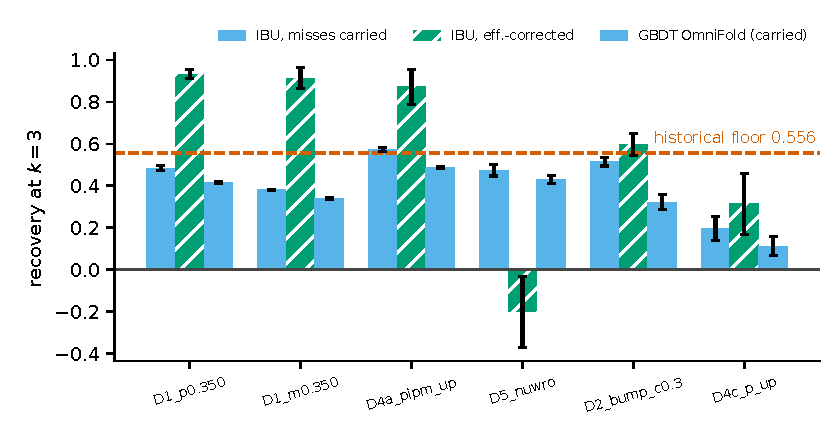
\includegraphics[width=0.95\linewidth]{figures_campaign/miss_tradeoff.pdf}
\end{column}
\end{columns}
\vspace{2pt}
{\footnotesize \textbf{Efficiency correction is far ahead when the distortion is a function of the variables the
unfolder sees, and it fails --- moves away from the target --- when the distortion changes the event mix
inside a truth bin}, because it extrapolates an acceptance that no longer holds. Carry-misses is slower
but does not fail that way. Neither mode is dominant: \textbf{the choice is a model-dependence choice and must
be stated as one.}}
\end{frame}

\gdef\evidencetext{\texttt{phase\_e/results/references.json}; \texttt{../configuration\_comparison/campaign\_report.json}}
\begin{frame}{Robustness (3): hidden variable and response scale}
\textbf{Hidden variable (D4d: neutron multiplicity up/down, invisible in $E_{\mathrm{avail}}$, visible to the
detector).} Every estimator ends farther from the target than the untouched prior: the projection on the injected
direction is negative (the wrong way) in 14 of 18 estimator $\times$ replicate
cells at $k=3$ (development tilt: positive in 9 of 9). This is the
hidden-variable limit any unfolding in these observables carries. That efficiency correction fails
\emph{specifically} worse here is \textbf{not established} at this sample size.\par\vspace{6pt}
\textbf{Detector response.} A $\pm5\,\%$ hadronic energy-scale error (R1) combined with the development tilt:
\begin{center}
{\footnotesize
\begin{tabular}{lrrr}
\toprule
estimator ($k=3$) & same response & R1 $\times$1.05 ($\Delta$) & R1 $\times$0.95 ($\Delta$) \\
\midrule
IBU, misses carried & 0.483 & 0.546 (+0.063) & 0.418 (\ensuremath{-}0.065) \\
GBDT OmniFold & 0.414 & 0.476 (+0.061) & 0.356 (\ensuremath{-}0.058) \\
\bottomrule
\end{tabular}}
\end{center}
Shifts average 0.06 in magnitude, 3.1\ensuremath{\times} the historical 0.02
non-inferiority margin. Same-response closure cannot see this: \textbf{any candidate's recovery statement is
conditional on the simulated response.}
\end{frame}

\gdef\evidencetext{\texttt{confirm/results/confirm\_results.json}}
\begin{frame}{The confirmatory result: pending}
\begin{alertblock}{Confirmatory results pending}
\small The FINAL comparison (fresh pool F, $n$ independent replicates) has not been harvested into
\texttt{confirm\_results.json}. No confirmatory decision,
superiority, non-inferiority or adequacy statement is made in this deck.
\end{alertblock}
{\scriptsize Frozen before any fresh-pool row was read (protocol amendment 2): \textbf{CTL} = historical recipe at $k=3$; \textbf{A} = the same run at $K^*=10$ (iterations alone); \textbf{B} = C2 inputs at $K^*$ (carry-misses); \textbf{C} = efficiency-corrected step 2 at $K^*$. Adequacy judged like-for-like at $k=3$ and at $K^*$ against the unchanged historical floors.}\par\vspace{2pt}

\begin{columns}[T]
\begin{column}{0.55\linewidth}
{\tiny
\begin{tabular}{lrrr}
\toprule
PILOT, pool P & P0 & P1 & P2 \\
\midrule
CTL (hist. recipe, $k=3$) & 0.297 & 0.329 & 0.349 \\
A (same run, $K^*=10$) & 0.457 & 0.508 & 0.501 \\
B (C2 inputs), $k=3$ & 0.454 & 0.455 & 0.504 \\
B (C2 inputs), $K^*=10$ & 0.542 & 0.551 & 0.539 \\
C (eff.-corr.), $k=3$ & 0.535 & 0.617 & --- \\
C (eff.-corr.), $K^*=10$ & 0.722 & 0.796 & --- \\
oracle anchor & 0.987 & 0.985 & 0.982 \\
\bottomrule
\end{tabular}}\par\vspace{2pt}
{\tiny FINAL sized from these at $n=12$ (uncapped 200; capped by pool F).}
\end{column}
\begin{column}{0.43\linewidth}
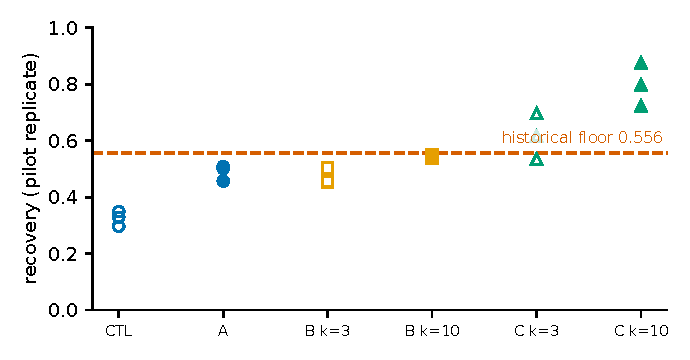
\includegraphics[width=0.95\linewidth]{figures_campaign/confirm_pilot.pdf}
\end{column}
\end{columns}
{\tiny \textbf{PILOT observations are not confirmatory.} They size FINAL and are reported separately;
they never enter the FINAL interval, and no decision is drawn from them.}
\end{frame}

\gdef\evidencetext{\texttt{PROTOCOL-20260922.md \S 1}; \texttt{../configuration\_comparison/campaign\_report.json}}
\begin{frame}{What a terminal result cannot authorize}
\begin{alertblock}{A terminal result of this campaign cannot authorize}
\begin{itemize}
\item adoption of any estimator for publication;
\item a change to the historical comparison's verdict (\texttt{NEITHER\_ELIGIBLE / NO\_SELECTION}, preserved) or to its thresholds;
\item $C_{\mathrm{stat}}$ / $C_{\mathrm{ML}}$ or any uncertainty product, any systematic, any central-value change,
any Gate-6 action;
\item any real-data unfolding.
\end{itemize}
\end{alertblock}
Recalibrated references and recommended configurations are \textbf{prospective recommendations only}.
Every result in this deck is from simulation: pseudodata built from signal Monte Carlo with a known
injected truth.\par\vspace{6pt}
\textbf{Scope.} PET is diagnostic method development. Nothing here is a publication adoption, and nothing here changes the historical comparison's verdict or thresholds.
\end{frame}

\gdef\evidencetext{\texttt{phase\_b/pet/results/summary.json}; \texttt{confirm/results/confirm\_results.json}}
\begin{frame}{Limitations and the next choice}
\textbf{Limitations}
\begin{itemize}\footnotesize
\item DEV-stage PET results rest on 2 seeds per arm. The repaired driver reproduces the historical recipe
(0.311 over 4 seeds, sd 0.03); effects below about that spread are
reported as unresolved, not as nulls.
\item Recovery statements are conditional on the simulated detector response (R1 moves them by more than the
margins) and cannot see hidden variables (D4d).
\item Efficiency correction needs a stopping rule and a variance statement, not only a mean recovery.
\item Coverage has not been run: protocol \S 7 reserves it for a candidate adequate or best-in-class on FINAL.
\end{itemize}
\textbf{Next choice}
\begin{itemize}\footnotesize
\item Confirmatory status: the FINAL comparison and the PET stress set are pending; until they land, every candidate statement above is development-stage evidence on the DEV halves.
\item The miss rule is a model-dependence choice (carry-misses: slower, does not move away; efficiency
correction: faster, fails when the event mix inside a truth bin changes). Whichever is recommended must be
stated as that choice.
\item A reference computed for the estimator's own miss rule and normalization, on the scored spectrum, is a
prospective recommendation to be checked on a known-function toy before use.
\end{itemize}
{\scriptsize \textbf{Scope.} PET is diagnostic method development. Nothing here is a publication adoption, and nothing here changes the historical comparison's verdict or thresholds.}
\end{frame}

\appendix
\gdef\evidencetext{}
\begin{frame}{Appendix}\centering\Large Backup\end{frame}

\gdef\evidencetext{\texttt{phase\_a/receipts/historical\_receipts.json}; \texttt{phase\_a/receipts/runtime\_audit\_theirs.json}}
\begin{frame}{Appendix: other executed facts (Phase A)}
\begin{itemize}\small
\item Every fit after iteration 0 ran at a forced learning rate (\ensuremath{1\times10^{-5}}), so the tuned rate governed iteration 0 only.
\item Early stopping was inert against 8 epochs: each fit handed on its \textbf{last-epoch} weights, while the
validation-loss minimum was the last epoch in only 7 of 48 final-stage fits for his arm and 30 of 48 for ours.
\item Step 1 normalizes each class to a fixed total, discarding the physical class ratio.
\item The step-2 truth cloud feeds \textbf{raw PDG codes} as a continuous column into Dense layers and the $k$-NN features.
\item \textbf{Not defective:} his pretrained weights survive cloning exactly (176 of 176 tensors at the first
optimizer step); his token features are the converted $\eta/\phi/\log p_T/\log E$ set.
\end{itemize}
\end{frame}

\gdef\evidencetext{\texttt{phase\_d/results/scalar\_scaling.json}}
\begin{frame}{Appendix: Phase D, all prior-size curves}
{\small Prior-MC size axis, mean $\pm$ sd over draws (Phase D, development stage):}
\begin{center}
{\scriptsize
\begin{tabular}{lrrrr}
\toprule
estimator & 75k & 150k & 300k & 600k \\
\midrule
OmniFold eff.-corrected, $k=3$ & 0.749 $\pm$ 0.043 & 0.748 $\pm$ 0.032 & 0.827 $\pm$ 0.021 & 0.793 $\pm$ 0.025 \\
AUSSIE, $\lambda=1000$ (misses pinned) & 0.679 $\pm$ 0.201 & 0.641 $\pm$ 0.083 & 0.663 $\pm$ 0.027 & 0.648 $\pm$ 0.031 \\
OmniFold carry-misses, $k=3$ & 0.337 $\pm$ 0.008 & 0.369 $\pm$ 0.022 & 0.411 $\pm$ 0.004 & 0.416 $\pm$ 0.009 \\
OmniFold carry-misses, $k=20$ & 0.447 $\pm$ 0.007 & 0.524 $\pm$ 0.072 & 0.582 $\pm$ 0.025 & 0.548 $\pm$ 0.012 \\
OmniFold eff.-corrected, $k=20$ & 0.794 $\pm$ 0.130 & 0.791 $\pm$ 0.051 & 0.862 $\pm$ 0.041 & 0.813 $\pm$ 0.042 \\
AUSSIE, $\lambda=0$ & 0.816 $\pm$ 0.024 & 0.820 $\pm$ 0.081 & 0.880 $\pm$ 0.043 & 0.849 $\pm$ 0.033 \\
\bottomrule
\end{tabular}}
\end{center}
{\small The efficiency-corrected and AUSSIE curves are flat in prior size: the signature of an estimator limited
by its extrapolation assumption rather than by statistics.}
\end{frame}

\gdef\evidencetext{\texttt{phase\_e/results/references.json}}
\begin{frame}{Appendix: Phase E scalar yardsticks, all predeclared cases}
{\small Predeclared truth distortions and R1 combined with the development tilt; mean recovery over 3 replicates,
fresh pool-T events.}
\begin{center}
{\tiny
\begin{tabular}{lrrrrrr}
\toprule
case & IBU carried $k$=3 & $k$=10 & IBU eff. $k$=3 & $k$=10 & GBDT $k$=3 & $k$=10 \\
\midrule
\texttt{D1\_m0.175} & 0.38 & 0.53 & 0.92 & 0.62 & 0.28 & 0.36 \\
\texttt{D1\_m0.350} & 0.38 & 0.52 & 0.91 & 0.78 & 0.34 & 0.43 \\
\texttt{D1\_m0.700} & 0.39 & 0.51 & 0.88 & 0.88 & 0.36 & 0.46 \\
\texttt{D1\_p0.175} & 0.45 & 0.62 & 0.88 & 0.79 & 0.34 & 0.41 \\
\texttt{D1\_p0.350} & 0.48 & 0.66 & 0.93 & 0.86 & 0.41 & 0.50 \\
\texttt{D1\_p0.700} & 0.56 & 0.74 & 0.96 & 0.86 & 0.51 & 0.60 \\
\texttt{D2\_bump\_c0.3} & 0.51 & 0.68 & 0.60 & 0.51 & 0.32 & 0.37 \\
\texttt{D2\_bump\_c1.0} & 0.35 & 0.51 & 0.54 & 0.52 & 0.22 & 0.30 \\
\texttt{D3\_m0.35} & 0.34 & 0.44 & 0.71 & 0.72 & 0.26 & 0.31 \\
\texttt{D3\_p0.35} & 0.40 & 0.51 & 0.68 & 0.58 & 0.32 & 0.37 \\
\texttt{D4a\_pipm\_down} & 0.50 & 0.63 & 0.87 & 0.66 & 0.40 & 0.47 \\
\texttt{D4a\_pipm\_up} & 0.57 & 0.71 & 0.87 & 0.78 & 0.49 & 0.56 \\
\texttt{D4b\_pi0\_down} & 0.51 & 0.67 & 0.84 & 0.54 & 0.38 & 0.47 \\
\texttt{D4b\_pi0\_up} & 0.56 & 0.74 & 0.92 & 0.76 & 0.46 & 0.54 \\
\texttt{D4c\_p\_down} & 0.29 & 0.41 & 0.26 & \ensuremath{-}0.40 & 0.20 & 0.20 \\
\texttt{D4c\_p\_up} & 0.20 & 0.19 & 0.31 & \ensuremath{-}0.40 & 0.11 & 0.13 \\
\texttt{D4d\_n\_down} & \ensuremath{-}0.41 & \ensuremath{-}0.90 & \ensuremath{-}1.95 & \ensuremath{-}4.91 & \ensuremath{-}0.06 & \ensuremath{-}0.09 \\
\texttt{D4d\_n\_up} & \ensuremath{-}0.32 & \ensuremath{-}0.59 & \ensuremath{-}0.46 & \ensuremath{-}2.12 & \ensuremath{-}0.15 & \ensuremath{-}0.15 \\
\texttt{D5\_fsi\_frabs} & 0.61 & 0.82 & 0.86 & 0.67 & 0.55 & 0.71 \\
\texttt{D5\_fsi\_frinel} & 0.61 & 0.81 & 0.86 & 0.67 & 0.56 & 0.71 \\
\texttt{D5\_genie\_mec} & 0.62 & 0.80 & 0.84 & 0.65 & 0.57 & 0.72 \\
\texttt{D5\_gibuu} & 0.55 & 0.69 & 0.65 & 0.50 & 0.44 & 0.50 \\
\texttt{D5\_nuwro} & 0.48 & 0.65 & \ensuremath{-}0.20 & \ensuremath{-}0.00 & 0.43 & 0.50 \\
\texttt{R1\_x0.95+D1\_p0.350} & 0.42 & 0.56 & 0.80 & 0.85 & 0.36 & 0.42 \\
\texttt{R1\_x1.05+D1\_p0.350} & 0.55 & 0.76 & 0.87 & 0.69 & 0.48 & 0.59 \\
\bottomrule
\end{tabular}}
\end{center}
\end{frame}

\gdef\evidencetext{\texttt{slides/deck\_numbers.json}}
\begin{frame}{Appendix: evidence files}
{\small Every number in this deck is read from these committed files by
\texttt{slides/make\_campaign\_deck.py}; \texttt{slides/deck\_numbers.json} records the field (or derivation)
behind each, and \texttt{slides/CLAIM\_INDEX-deck.md} maps every claim to them. Paths relative to
\texttt{nd-unfolding/pet/improvement\_campaign/}; sha256 prefixes.}
\begin{center}
{\tiny
\begin{tabular}{ll}
\toprule
file & sha256 \\
\midrule
\texttt{../configuration\_comparison/campaign\_report.json} & \texttt{96955a10222b6c95} \\
\texttt{confirm/results/confirm\_results.json} & \texttt{4a00848e37a08f67} \\
\texttt{phase\_a/receipts/historical\_receipts.json} & \texttt{938b97521cc77e82} \\
\texttt{phase\_a/receipts/runtime\_audit\_theirs.json} & \texttt{8dadb3f32d3fec72} \\
\texttt{phase\_b/pet/results/summary.json} & \texttt{ed81c51f67e9df24} \\
\texttt{phase\_b/scalar/results/reference\_decomposition.json} & \texttt{aa831560259f1255} \\
\texttt{phase\_b/scalar/results/summary.json} & \texttt{50665f198fa4ad73} \\
\texttt{phase\_d/results/scalar\_scaling.json} & \texttt{a0eadf592dc8e42a} \\
\texttt{phase\_e/results/identifiability.json} & \texttt{856aa31aae209fe8} \\
\texttt{phase\_e/results/reference\_assessment.json} & \texttt{610e643515efbc34} \\
\texttt{phase\_e/results/references.json} & \texttt{5c27d2ce21097102} \\
\texttt{phase\_e/results/toy\_reference.json} & \texttt{dd5d85c699adbd3d} \\
\texttt{phase\_f/results/aussie\_ablation.json} & \texttt{cbe81805d792468e} \\
\bottomrule
\end{tabular}}
\end{center}
{\tiny Plus 16 per-run PET score files under \texttt{phase\_b/pet/results/} (hashes in
\texttt{deck\_numbers.json}).}
\end{frame}

\end{document}
